% Tutto quello riguardante il progetto andrà in questo capitolo 

\chapter{Tecnologie utilizzate}\label{chap:tec}
\section{Ambiente di sviluppo}
\subsection{Docker}
	\begin{figure}[H] 
		\centering
		
\includegraphics[scale=0.3]{loghi/docker}
		\caption{Logo Docker}
	\end{figure}
Docker è una piattaforma per lo sviluppo, rilascio ed esecuzione di applicazione 
all'interno di \emph{container}. Questi ultimi forniscono una virtualizzazione a livello 
del sistema operativo \emph{Linux} senza che sia necessario istanziare delle macchine 
virtuali pienamente operative.
I \emph{container} sono assimilabili a delle macchine virtuali modulari con la peculiarità 
di essere molto leggere: in questo modo risulta più facile creare, distribuire, 
copiare e spostare i container da un ambiente all'altro.
Ogni \emph{container} è un processo isolato dagli altri \emph{container} e dal sistema ospite stesso: ogni volta che viene istanziato un nuovo \emph{container} si avrà un ambiente pulito, ovvero indipendente dal sistema ospite, da \emph{container} precedentemente creati e con le caratteristiche specificate. \\
Per sviluppare l'applicazione \emph{Teamwork} è stato utilizato \emph{Docker 18.03 Community Edition} per \emph{Ubuntu Bionic}. In questo modo si è potuto instanziare nelle macchine locali un \emph{container} di \emph{Zimbra} e del \emph{core Zextras} con la \emph{zimlet OpenChat} caricata così da sviluppare l'applicativo in un ambiente sicuro e pulito.

\subsection{IntelliJ IDEA} \label{subsec:IntelliJ}
	\begin{figure}[H] 
		\centering
		
\includegraphics[scale=0.2]{loghi/intellij-idea}
		\caption{Logo IntelliJ IDEA}
	\end{figure}
IntelliJ IDEA è un \emph{\textbf{I}ntegrated \textbf{D}evelopment \textbf{E}nvironment} (\acrshort{IDE}) multi-linguaggio e multi-piattaforma. 
È stata utilizzata l'edizione \emph{Ultimate} in quanto era necessario un editor che 
supportasse JavaScript/TypeScript, mentre la \emph{Community edition} non supporta questi linguaggi. 
Dovendo creare un'applicazione con numerose referenze al codice della \emph{zimlet 
OpenChat} e di \emph{Zimbra} sono state sfruttate al meglio le funzionalità per 
analizzare il codice e comprendere le dipendenze esistenti.

\subsection{Expo} \label{subsec:expo}
	\begin{figure}[H] 
		\centering
		
\includegraphics[scale=0.05]{loghi/expo}
		\caption{Logo Expo}
	\end{figure}
Expo è una \emph{toolchain} \emph{open source} che permette la gestione di un progetto React Native utilizzando il \emph{\textbf{S}oftware \textbf{D}evelopment \textbf{K}it} (\acrshort{SDK}) di Expo. L'SDK Expo è una libreria nativa e JavaScript 
che fornisce l'accesso alle funzionalità del sistema del dispositivo (come la 
fotocamera, i contatti, la memoria locale) senza il bisogno di utilizzare \gl{xCode}{xCode} 
o \gl{Android Studio}{Android Studio}, né di utilizzare codice nativo. Fornisce l'accesso a servizi 
che in genere sono difficili da gestire nativamente, ma sono richiesti da quasi 
tutte le app come le notifiche \emph{push} o creare binari nativi pronti per la 
distribuzione nell'\emph{app store}.
Inoltre risulta molto facile lo sviluppo e il test dato che permette delle 
\emph{build} automatiche nei loro \emph{server} che possono eseguire in \emph{real-time} il codice 
sia in simulatori che in dispositivi mobili.


\section{Linguaggi, librerie e strumenti di programmazione}

\subsection{React Native}
\begin{figure}[H] 
	\centering
	
\includegraphics[scale=0.1]{loghi/React}
	\caption{Logo React Native}
\end{figure}
React Native è un \emph{framework} per lo sviluppo di applicazioni mobile in JavaScript 
permettendo di unificare l'esperienza di sviluppo su diversi sistemi operativi. 
Infatti React Native utilizza gli stessi le stesse componenti dell'interfaccia 
utente che vengono utilizzate da app native iOS e Android.
Si possono comunque integrare dei componenti scritti in \emph{Objective-C}, 
\emph{Java} o \emph{Swift} così da passare al codice nativo nel caso fosse necessario 
ottimizzare alcuni aspetti dell'applicazione in base alla piattaforma. 
React Native si basa su ReactJS dove appare fondamentale il concetto di 
componente. Un componente è un modulo dell'applicazione che ha uno stato, 
che può accettare delle proprietà e che ha un proprio ciclo di vita. 
Questo approccio di sviluppo atomico risulta perfetto per effettuare Unit Test 
o per creare componenti più complessi includendone altri più semplici.

\subsection{TypeScript} \label{subsec:tslint}
\begin{figure}[H] 
	\centering
	
\includegraphics[scale=0.07]{loghi/ts}
	\caption{Logo TypeScript}
\end{figure}
TypeScript è un linguaggio di programmazione sviluppato da \emph{Microsoft} che 
estende la sintassi di JavaScript.  È nato per poter utilizzare le funzionalità di 
JavaScript per lo sviluppo di grandi applicazioni in quanto ne aumenta la 
sicurezza e la robustezza del codice tramite l'aggiunta di classi, interfacce, 
moduli, tipizzazione e altre funzionalità importanti per la comprensione di un 
grande progetto. 
Il codice TypeScript sviluppato viene successivamente ricompilato in JavaScript 
per poter essere interpretato da browser o app.

\subsection{TSLint}
\begin{figure}[H] 
	\centering
	
\includegraphics[scale=0.4]{loghi/TSlint}
	\caption{Logo TS Lint}
\end{figure}
TSLint è uno strumento di \gl{analisi statica}{analisi statica} per il codice scritto in TypeScript 
che offre funzionalità estendibili e personalizzabili per la leggibilità, la 
manutenibilità e gli errori di funzionalità. 
È supportato da molti dei moderni editor, compreso \emph{IntelliJ IDEA} (sez. 
\ref{subsec:IntelliJ}), utilizzato per il progetto.

\subsection{Redux} \label{subsec:Redux}
\begin{figure}[H] 
	\centering
	
\includegraphics[scale=0.06]{loghi/redux}
	\caption{Logo Redux}
\end{figure}
Redux è una libreria JavaScript per la gestione semplificata dello stato delle 
applicazioni web. In ReactJS e React Native ogni componente possiede uno stato 
che può cambiare durante il suo ciclo di vita. Questo stato è interno ad ogni 
singola componente ed è difficile, a volte impossibile, la comunicazione di questi 
dati tra componenti diverse. 
Redux, invece, permette la creazione di uno \emph{store} condiviso, accessibile da tutte 
le componenti. In tal modo è possibile sincronizzare le modifiche e quindi 
avere dei dati coerenti tra le varie componenti. 
Redux è stato implementato basandosi su una particolare architettura: 
\hyperref[subsec:flux]{Flux}.

\subsubsection{Flux} \label{subsubsec:flux}
 Flux è un \gl{pattern architetturale}{pattern architetturale} che ha ispirato Redux, utilizzato per la 
 creazione di applicazioni web \emph{client-side}. Esso utilizza un flusso di dati 
 unidirezionale per gestire al meglio la sincronizzazione degli stati tra le 
 componenti React. In questo modo si è sicuri che lo stato dello \emph{store} sia 
 sempre uguale in tutte le componenti che compongono la \emph{view}.
 
 \begin{figure}[H] 
 	\centering
 	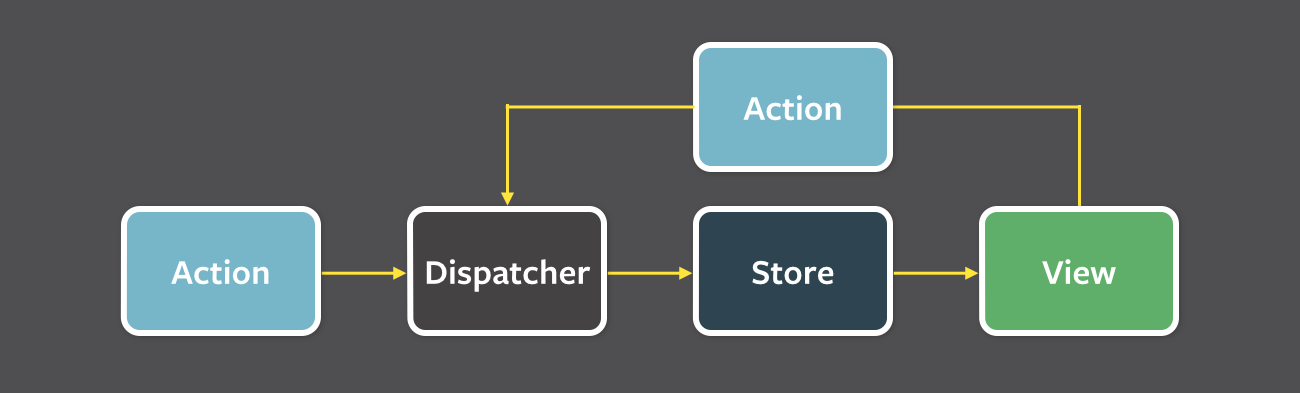
\includegraphics[scale=0.3]{loghi/flux}
 	\caption{Flusso dei dati in Flux}
 \end{figure}
 Il flusso parte da degli oggetti \emph{stores}, che contengono i dati dell’applicazion che vengono forniti ai componenti dell'applicazione in modo che la view sia sempre aggiornata con questi dati. \\
Per modificare i dati presenti in uno store è necessario creare un oggetto \emph{action} che, mediante il \emph{dispatcher} dell’applicazione, viene ricevuto dai vari \emph{stores}, i quali lo utilizzano per aggiornare i dati che contengono.

 
\section{Strumenti di verifica e valutazione}

\subsection{Genymotion} \label{subsez:genymotion}
\begin{figure}[H] 
	\centering
	
\includegraphics[scale=0.2]{loghi/genymotion2}
	\caption{Logo Genymotion}
\end{figure}
Genymotion è un emulatore software di dispositivi Android. Si integra 
perfettamente con Expo(sez. \ref{subsec:expo}) utilizzato per la gestione di 
questo progetto, permettendo di avere un riscontro dell'app in \emph{real-time} durante 
lo sviluppo e di verificare e testare l'applicazione su più \emph{device}. Emula più 
di 3000 configurazioni virtuali di dispositivi Android (tra versioni, dimensioni 
schermo, capacità hardware, ecc..). 

\subsection{React Native Debugger}
\begin{figure}[H] 
	\centering
	
\includegraphics[scale=0.15]{loghi/react-native-debugger}
	\caption{Logo React Native Debugger}
\end{figure}
React Native Debugger è un applicazione \emph{standalone} per il \emph{debug} di app in React 
Native. Si basa sul remote dedugger disponibile quando si monitora un progetto 
in un device fisico o virtuale.
\newpage
Esso offre vari strumenti per il debug:
\begin{itemize}
	\item \textbf{React Inspecto}r, per ispezionare il \emph{layout} e lo \emph{style} di ogni componente dell'app;
	\item \textbf{Redux DevTools}, per monitorare gli \emph{store} Redux utilizzati e le \emph{action} svolte su di essi;
	\item \textbf{Console}, per visualizzare errori e avvisi che avvengono durante l'esecuzione del codice.
\end{itemize}

\subsection{Jest} \label{subsez:jest}
\begin{figure}[H] 
	\centering
	
\includegraphics[scale=0.13]{loghi/jest}
	\caption{Logo Jest}
\end{figure}
Jest è un framework di \gl{unit testing}{unit testing} per JavaScript sviluppato ed utilizzato da 
\emph{Facebook} per testare le proprie applicazioni in React. È una soluzione completa 
e pronta in quanto è automaticamente configurata alla creazione di un progetto 
React Native.
Rispetto ad altri framework di unit testing offre dei vantaggi, come: 
\begin{itemize}
	\item vengono eseguiti solo i file di test relativi ai file modificati;
	\item gestisce automaticamente le dipendenze durante l'esecuzione dei test;
	\item permette di testare in modo sincroni il codice asincrono;
	\item esegue i test in processi paralleli così che finiscano prima.
\end{itemize}
Inoltre Jest funziona con qualsiasi linguaggio \emph{compile-to-JavaScript}. 
Sia il codice da testare che i test stessi possono essere scritti in TypeScript, 
linguaggio utilizzato per questo progetto. 
